
\documentclass[11pt]{article}

\usepackage[margin=0.85in]{geometry}
\usepackage{amsmath,amssymb}
\usepackage{enumitem}
\usepackage{xcolor}
\usepackage{tcolorbox}
\usepackage{fancyhdr}
\usepackage{lastpage}
\usepackage{hyperref}
\usepackage{microtype}
\usepackage{tikz}

\definecolor{uwpurple}{HTML}{4B2E83}
\definecolor{uwgold}{HTML}{B7A57A}
\definecolor{softpurple}{HTML}{F4F1FA}
\definecolor{softgold}{HTML}{FBF7EA}
\definecolor{deepgold}{HTML}{8A6F2A}

\tcbuselibrary{breakable,skins}

\newtcolorbox{solutionbox}[1][]{
    breakable,
    enhanced,
    colback=softgold,
    colframe=deepgold,
    coltitle=white,
    colbacktitle=uwpurple,
    fonttitle=\bfseries,
    title={Solution #1},
    boxrule=0.85pt,
    arc=2mm,
    left=2.5mm,
    right=2.5mm,
    top=1.5mm,
    bottom=1.5mm,
    attach boxed title to top left={xshift=2.5mm,yshift=-2mm},
    boxed title style={
        colback=uwpurple,
        colframe=uwpurple,
        arc=1.5mm,
        boxrule=0pt,
        left=1.6mm,
        right=1.6mm,
        top=0.6mm,
        bottom=0.6mm
    }
}

\newtcolorbox{finalanswerbox}[1][]{
    breakable,
    colback=white,
    colframe=uwpurple,
    boxrule=0.75pt,
    arc=2mm,
    left=2mm,
    right=2mm,
    top=1mm,
    bottom=1mm,
    title={\textbf{Final Answer #1}},
    coltitle=uwpurple,
    colbacktitle=softpurple,
    fonttitle=\bfseries
}

\hypersetup{colorlinks=true, linkcolor=uwpurple, urlcolor=uwpurple}

\pagestyle{fancy}
\fancyhf{}
\lhead{\textbf{MATH 394: Probability I}}
\rhead{\textbf{Homework 7 Solutions}}
\cfoot{\thepage\ of \pageref{LastPage}}

\setlength{\parindent}{0pt}
\setlength{\parskip}{0.45em}

\newcommand{\course}{MATH 394: Probability I}
\newcommand{\instructor}{Arman Jahangiri}
\newcommand{\department}{Department of Mathematics}
\newcommand{\university}{University of Washington}

\newtcolorbox{problemheader}{
    colback=softpurple,
    colframe=uwpurple,
    boxrule=0.8pt,
    arc=2mm,
    left=2mm,
    right=2mm,
    top=1mm,
    bottom=1mm
}

\newcommand{\source}[2]{%
    \vspace{0.15cm}
    {\small\textit{Source: Blitzstein and Hwang, \textit{Introduction to Probability}, Chapter #1, Problem #2.}}
}

\begin{document}

\begin{titlepage}
\centering
\vspace*{1.2cm}

{\Large \textbf{\university}}\\
{\large \department}

\vspace{1.5cm}

{\Huge \color{uwpurple}\textbf{Homework 7 Solutions}}\\[0.25cm]
{\Large \textbf{\course}}\\[0.25cm]
{\large Instructor: Arman Jahangiri}

\vspace{1cm}

\begin{tcolorbox}[width=0.78\textwidth,colback=softpurple,colframe=uwpurple,boxrule=0.9pt,arc=3mm]
\centering
\textbf{Submission:} Single PDF on Gradescope

\textbf{Deadline:} 10:00 PM Pacific Time on the listed due date
\end{tcolorbox}

\vspace{0.8cm}

\begin{tcolorbox}[width=0.86\textwidth,colback=white,colframe=uwgold,boxrule=0.8pt,arc=3mm]
This homework is worth \textbf{50 points}.

Across the quarter, there are \textbf{eight homework assignments}, worth \textbf{400 points total}. Homework assignments together account for \textbf{40\%} of the final course grade. Further course policies can be seen in the \href{https://armanjg.github.io/MATH-394-Probability-1/}{\textbf{MATH 394 syllabus}.}
\end{tcolorbox}

\vfill
\end{titlepage}

\section*{Homework Policy}

\subsection*{Submission and Deadline}

Please:

\begin{itemize}[leftmargin=*]
    \item Submit homework as a single PDF on Gradescope by \textbf{10:00 PM (Pacific Time)} on the listed due date.
    \item Begin each problem on a new page, and ensure that pages are correctly tagged in Gradescope.
    \item Write solutions clearly and legibly.
    \item Typesetting solutions in LaTeX is encouraged, but not required.
\end{itemize}

\subsection*{Late Days}

Each student is allotted \textbf{six late days} for the quarter. A late day extends a homework deadline by up to 24 hours without penalty. For example, submitting an assignment anytime between 10:01 PM on the due date and 10:00 PM the following day counts as one late day.

The following rules apply:
\begin{itemize}[leftmargin=*]
   \item No explanation is required to use late days.
   \item At most \textbf{two late days} may be used on any single homework assignment.
   \item Late days may not be used on the final homework assignment or on any assignment for which solutions have already been released.
   \item It is the student's responsibility to keep track of how many late days have been used during the quarter.
\end{itemize}

Once all late days have been exhausted, additional late submissions will incur a penalty of \textbf{10\% per day}, up to a maximum deduction of \textbf{50\%}. Assignments submitted more than five days late, or after solutions have been released, will not be accepted.

\subsection*{Submission Issues and Technical Difficulties}

If a serious technical issue prevents a timely Gradescope submission, students may temporarily submit their assignment by email to the instructor at \href{mailto:armanjg@uw.edu}{armanjg@uw.edu}. In such cases:

\begin{itemize}[leftmargin=*]
    \item The submission must consist of a \textbf{single PDF file}. The email subject line must follow the format:
    \[
    \texttt{HW\# Submission - FULL NAME - STUDENT ID}.
    \]
    \item Once the Gradescope issue has been resolved, the student must upload the \emph{exact same file} to Gradescope as soon as possible.
    \item The student should clearly indicate in the Gradescope submission that the assignment was previously submitted by email before the deadline.
\end{itemize}

Email submissions are intended only for genuine technical emergencies and should not be used as a substitute for timely Gradescope submission.

\newpage

% ------------------------------------------------------------
\begin{problemheader}
\textbf{Problem 1.  }
\end{problemheader}
\source{7}{1}

Alice and Bob arrange to meet for lunch on a certain day at noon. However, neither is known for punctuality. They both arrive independently at uniformly distributed times between noon and 1 pm on that day. Each is willing to wait up to 15 minutes for the other to show up.

What is the probability they will meet for lunch that day?

\begin{solutionbox}
Measure arrival times in hours after noon, and let Alice's and Bob's arrival times be
\[
X,Y\sim \operatorname{Unif}(0,1),
\]
independently.

Since \(X\) and \(Y\) are independent and each has density
\[
f_X(x)=f_Y(y)=1,
\qquad 0\le x,y\le 1,
\]
their joint density is
\[
f_{X,Y}(x,y)
=
f_X(x)f_Y(y)
=
\begin{cases}
1, & 0\le x\le 1,\;0\le y\le 1,\\
0, & \text{otherwise}.
\end{cases}
\]

They meet exactly when their arrival times differ by at most 15 minutes, or \(1/4\) of an hour. Thus
\[
|X-Y|\le \frac14.
\]

Therefore,
\[
\mathbb P\left(|X-Y|\le \frac14\right)
=
\iint_{\{|x-y|\le 1/4\}} f_{X,Y}(x,y)\,dy\,dx.
\]

For a fixed \(x\), the condition
\[
|x-y|\le \frac14
\]
is equivalent to
\[
x-\frac14\le y\le x+\frac14.
\]
Taking into account that \(0\le y\le 1\), we split the integral into three parts:
\[
\begin{aligned}
\mathbb P\left(|X-Y|\le \frac14\right)
&=
\int_0^{1/4}\int_0^{x+1/4} 1\,dy\,dx\\
&\quad+
\int_{1/4}^{3/4}\int_{x-1/4}^{x+1/4} 1\,dy\,dx\\
&\quad+
\int_{3/4}^{1}\int_{x-1/4}^{1} 1\,dy\,dx.
\end{aligned}
\]

Evaluating,
\[
\begin{aligned}
\mathbb P\left(|X-Y|\le \frac14\right)
&=
\int_0^{1/4}\left(x+\frac14\right)\,dx
+
\int_{1/4}^{3/4}\frac12\,dx
+
\int_{3/4}^{1}\left(\frac54-x\right)\,dx\\
&=
\frac{3}{32}
+
\frac14
+
\frac{3}{32}\\
&=
\frac{7}{16}.
\end{aligned}
\]

\end{solutionbox}
\newpage

% ------------------------------------------------------------

\begin{problemheader}
\textbf{Problem 2.  }
\end{problemheader}
\source{7}{7}

A stick of length $L$, where $L$ is a positive constant, is broken at a uniformly random point $X$. Given that $X=x$, another breakpoint $Y$ is chosen uniformly on the interval $[0,x]$.

\begin{enumerate}[label=(\alph*), leftmargin=*]
    \item Find the joint PDF of $X$ and $Y$. Be sure to specify the support.

    \item We already know that the marginal distribution of $X$ is $\operatorname{Unif}(0,L)$. Check that marginalizing out $Y$ from the joint PDF agrees that this is the marginal distribution of $X$.

    \item We already know that the conditional distribution of $Y$ given $X=x$ is $\operatorname{Unif}(0,x)$. Check that using the definition of conditional PDFs agrees that this is the conditional distribution of $Y$ given $X=x$.

    \item Find the marginal PDF of $Y$.

    \item Find the conditional PDF of $X$ given $Y=y$.
\end{enumerate}

\begin{solutionbox}
\textbf{(a)} Since \(X\sim \operatorname{Unif}(0,L)\), we have
\[
f_X(x)=\frac1L,\qquad 0<x<L.
\]
Given \(X=x\), the random variable \(Y\) is uniform on \((0,x)\), so
\[
f_{Y\mid X}(y\mid x)=\frac1x,\qquad 0<y<x.
\]
Thus
\[
f_{X,Y}(x,y)=f_X(x)f_{Y\mid X}(y\mid x)=\frac{1}{Lx},
\qquad 0<y<x<L.
\]
It is zero outside this region.
 

\textbf{(b)} Marginalizing out \(Y\), for \(0<x<L\), gives
\[
f_X(x)=\int_0^x \frac{1}{Lx}\,dy=\frac{1}{Lx}\cdot x=\frac1L.
\]
This is exactly the \(\operatorname{Unif}(0,L)\) density.


\textbf{(c)} Using the definition of a conditional density,
\[
f_{Y\mid X}(y\mid x)=\frac{f_{X,Y}(x,y)}{f_X(x)}
=\frac{1/(Lx)}{1/L}=\frac1x,
\qquad 0<y<x.
\]
This is the uniform density on \((0,x)\), as expected.
 

\textbf{(d)} For a fixed \(y\), the possible values of \(x\) run from \(y\) to \(L\). Hence, for \(0<y<L\),
\[
f_Y(y)=\int_y^L \frac{1}{Lx}\,dx
=\frac1L\log\left(\frac{L}{y}\right).
\]
 

\textbf{(e)} Finally,
\[
f_{X\mid Y}(x\mid y)
=\frac{f_{X,Y}(x,y)}{f_Y(y)}
=\frac{1/(Lx)}{(1/L)\log(L/y)}
=\frac{1}{x\log(L/y)},
\]
for \(y<x<L\).

 
\end{solutionbox}
\newpage

% ------------------------------------------------------------
 
\begin{problemheader}
\textbf{Problem 3.}
\end{problemheader}
\source{7}{15}

Let $X$ and $Y$ be continuous random variables, with joint CDF $F(x,y)$. Show that the probability that $(X,Y)$ falls into the rectangle $[a_1,a_2]\times[b_1,b_2]$ is
\[
F(a_2,b_2)-F(a_1,b_2)+F(a_1,b_1)-F(a_2,b_1).
\]

\begin{solutionbox}
\textit{We have covered this fully in the lecture with a visual representation (Lecture 19). }

Recall that the joint CDF of $X$ and $Y$ is
$$
F(x,y)=P(X\le x,\;Y\le y).
$$

Since $X$ and $Y$ are continuous, let $f_{X,Y}$ denote their joint density. It is related to the joint CDF by
$$
f_{X,Y}(x,y)
=
\frac{\partial^2}{\partial x\,\partial y}F(x,y).
$$

The probability that $(X,Y)$ falls inside the rectangle
$$
[a_1,a_2]\times[b_1,b_2]
$$
is therefore
$$
P(a_1\le X\le a_2,\;b_1\le Y\le b_2)
=
\int_{a_1}^{a_2}\int_{b_1}^{b_2}
f_{X,Y}(x,y)\,dy\,dx.
$$

Substituting
$$
f_{X,Y}(x,y)
=
\frac{\partial^2}{\partial x\,\partial y}F(x,y),
$$
we obtain
$$
\begin{aligned}
P(a_1\le X\le a_2,\;b_1\le Y\le b_2)
&=
\int_{a_1}^{a_2}
\int_{b_1}^{b_2}
\frac{\partial^2}{\partial x\,\partial y}F(x,y)
\,dy\,dx.
\end{aligned}
$$

First integrate with respect to $y$:
$$
\begin{aligned}
&=
\int_{a_1}^{a_2}
\left[
\frac{\partial}{\partial x}F(x,y)
\right]_{y=b_1}^{y=b_2}
dx\\
&=
\int_{a_1}^{a_2}
\left(
\frac{\partial}{\partial x}F(x,b_2)
-
\frac{\partial}{\partial x}F(x,b_1)
\right)dx.
\end{aligned}
$$

Now integrate with respect to $x$:
$$
\begin{aligned}
&=
\left[F(x,b_2)\right]_{a_1}^{a_2}
-
\left[F(x,b_1)\right]_{a_1}^{a_2}\\
&=
\left(F(a_2,b_2)-F(a_1,b_2)\right)
-
\left(F(a_2,b_1)-F(a_1,b_1)\right).
\end{aligned}
$$

Hence,
$$
P(a_1\le X\le a_2,\;b_1\le Y\le b_2)
=
F(a_2,b_2)-F(a_1,b_2)
-F(a_2,b_1)+F(a_1,b_1).
$$

\medskip

\textbf{Visual reasoning.}

Recall that
$$
F(a_2,b_2)
$$
represents all probability mass in the region
$$
X\le a_2,
\qquad
Y\le b_2.
$$

Think of this as one large lower-left rectangle extending up to
$$
(a_2,b_2).
$$

We only want the smaller rectangle
$$
a_1\le X\le a_2,
\qquad
b_1\le Y\le b_2.
$$

Starting from
$$
 {F(a_2,b_2)},
$$
we remove the part to the left of $a_1$:
$$
- {F(a_1,b_2)},
$$
and remove the part below $b_1$:
$$
- {F(a_2,b_1)}.
$$

However, the lower-left corner
$$
X\le a_1,
\qquad
Y\le b_1
$$
was contained in both of the pieces we subtracted, so it has been
subtracted twice. We therefore add it back once:
$$
+ {F(a_1,b_1)}.
$$

Thus the desired rectangle is obtained by the two-dimensional
inclusion--exclusion rule:
$$
 {
\text{desired rectangle}
=
\text{large rectangle}
-\text{left rectangle}
-\text{bottom rectangle}
+\text{overlap}.
}
$$
  





\begin{center}
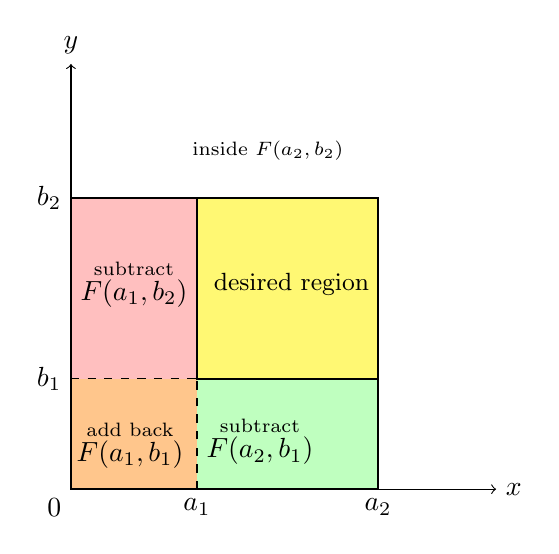
\begin{tikzpicture}[scale=5]

% parameters
\def\aone{0.32}
\def\atwo{0.78}
\def\bone{0.28}
\def\btwo{0.74}

% axes
\draw[->] (0,0) -- (1.08,0) node[right] {$x$};
\draw[->] (0,0) -- (0,1.08) node[above] {$y$};

% big rectangle corresponding to F(a2,b2)
\fill[blue!10] (0,0) rectangle (\atwo,\btwo);

% left part to subtract: F(a1,b2)
\fill[red!25] (0,0) rectangle (\aone,\btwo);

% bottom part to subtract: F(a2,b1)
\fill[green!25] (0,0) rectangle (\atwo,\bone);

% overlap added back: F(a1,b1)
\fill[orange!45] (0,0) rectangle (\aone,\bone);

% desired rectangle
\fill[yellow!55] (\aone,\bone) rectangle (\atwo,\btwo);

% outlines
\draw[thick] (0,0) rectangle (\atwo,\btwo);
\draw[thick] (\aone,\bone) rectangle (\atwo,\btwo);

% guide lines
\draw[dashed] (\aone,0) -- (\aone,\btwo);
\draw[dashed] (\atwo,0) -- (\atwo,\btwo);
\draw[dashed] (0,\bone) -- (\atwo,\bone);
\draw[dashed] (0,\btwo) -- (\atwo,\btwo);

% axis labels
\node[below] at (\aone,0) {$a_1$};
\node[below] at (\atwo,0) {$a_2$};
\node[left] at (0,\bone) {$b_1$};
\node[left] at (0,\btwo) {$b_2$};

% corner labels
\node[below left] at (0,0) {$0$};

% annotations
\node at (0.56,0.52) {\small desired region};
\node[align=center] at (0.16,0.52) {\scriptsize subtract\\[-1mm] $F(a_1,b_2)$};
\node[align=center] at (0.48,0.12) {\scriptsize subtract\\[-1mm] $F(a_2,b_1)$};
\node[align=center] at (0.15,0.11) {\scriptsize add back\\[-1mm] $F(a_1,b_1)$};

% label for big rectangle
\node[align=center] at (0.50,0.86) {\scriptsize inside $F(a_2,b_2)$};

\end{tikzpicture}
\end{center}
 
\end{solutionbox}

\newpage

% ------------------------------------------------------------

\begin{problemheader}
\textbf{Problem 4.  }
\end{problemheader}
\source{7}{16}

Let $X$ and $Y$ have joint PDF
\[
f_{X,Y}(x,y)=x+y,\qquad 0<x<1,\;0<y<1.
\]

\begin{enumerate}[label=(\alph*), leftmargin=*]
    \item Check that this is a valid joint PDF.

    \item Are $X$ and $Y$ independent?

    \item Find the marginal PDFs of $X$ and $Y$.

    \item Find the conditional PDF of $Y$ given $X=x$.
\end{enumerate}

\begin{solutionbox}
\textbf{(a)} First, note that if $x,y \in (0,1)$, then $f_{X,Y}(x,y) = x+y\geq 0$. Otherwise, $f_{X,Y}(x,y) = 0\geq 0$. So overall, $f_{X,Y}(x,y)\geq0 \ \ \forall x,y\in \mathbb{R}$.


Its total integral is
\[
\int_0^1\int_0^1 (x+y)\,dy\,dx
=
\int_0^1\left(x+\frac12\right)dx
=\frac12+\frac12=1.
\]
Thus it is a valid joint PDF.
 

\textbf{(b)} The variables are not independent. One way to see this is to compute the marginals and observe that their product does not equal the joint density.
 

\textbf{(c)} For \(0<x<1\),
\[
f_X(x)=\int_0^1 (x+y)\,dy=x+\frac12.
\]
Similarly, for \(0<y<1\),
\[
f_Y(y)=\int_0^1 (x+y)\,dx=y+\frac12.
\]
 

\textbf{(d)} For \(0<x<1\), the conditional density is
\[
f_{Y\mid X}(y\mid x)
=\frac{f_{X,Y}(x,y)}{f_X(x)}
=\frac{x+y}{x+1/2},
\qquad 0<y<1.
\]
 
\end{solutionbox}
\newpage

% ------------------------------------------------------------

\begin{problemheader}
\textbf{Problem 5. }
\end{problemheader}
\source{7}{17}

Let $X$ and $Y$ have joint PDF
\[
f_{X,Y}(x,y)=cxy,\qquad 0<x<y<1.
\]

\begin{enumerate}[label=(\alph*), leftmargin=*]
    \item Find $c$ to make this a valid joint PDF.

    \item Are $X$ and $Y$ independent?

    \item Find the marginal PDFs of $X$ and $Y$.

    \item Find the conditional PDF of $Y$ given $X=x$.
\end{enumerate}

\begin{solutionbox}
\textbf{(a)} We need
\[
\int_0^1\int_0^y cxy\,dx\,dy=1.
\]
The integral is
\[
c\int_0^1 y\left(\int_0^y x\,dx\right)dy
=
c\int_0^1 y\cdot \frac{y^2}{2}\,dy
=
\frac{c}{2}\cdot \frac14
=
\frac{c}{8}.
\]
Thus \(c=8\).
 

\textbf{(b)} The variables are not independent. The support itself already shows this, since the condition \(0<X<Y<1\) ties the possible values of \(X\) and \(Y\) together.
 

\textbf{(c)} With \(c=8\), for \(0<x<1\),
\[
f_X(x)=\int_x^1 8xy\,dy=4x(1-x^2).
\]
For \(0<y<1\),
\[
f_Y(y)=\int_0^y 8xy\,dx=4y^3.
\]
 

\textbf{(d)} For fixed \(x\), the conditional support is \(x<y<1\). Therefore
\[
f_{Y\mid X}(y\mid x)
=\frac{8xy}{4x(1-x^2)}
=\frac{2y}{1-x^2},
\qquad x<y<1.
\]
 
\end{solutionbox}
\newpage

% ------------------------------------------------------------
\begin{problemheader}
\textbf{Problem 6.}
\end{problemheader}
\source{7}{21}

Find the probability that the quadratic polynomial
$$
Ax^2+Bx+1,
$$
where the coefficients $A$ and $B$ are determined by drawing i.i.d. $\operatorname{Unif}(0,1)$ random variables, has at least one real root.

\emph{Hint: By the quadratic formula, the polynomial $ax^2+bx+c$ has a real root if and only if $b^2-4ac\ge0$.}

\begin{solutionbox}

A quadratic polynomial $Ax^2+Bx+1$ has at least one real root if and only if its discriminant is nonnegative. Therefore,
$$
B^2-4A\ge 0.
$$

Equivalently,
$$
A\le \frac{B^2}{4}.
$$

Since
$$
A,B\overset{\text{i.i.d.}}{\sim}\operatorname{Unif}(0,1),
$$
their marginal densities are
$$
f_A(a)=
\begin{cases}
1, & 0\le a\le 1,\\
0, & \text{otherwise},
\end{cases}
\qquad
f_B(b)=
\begin{cases}
1, & 0\le b\le 1,\\
0, & \text{otherwise}.
\end{cases}
$$

Because $A$ and $B$ are independent, their joint density is
$$
f_{A,B}(a,b)
=
f_A(a)f_B(b)
=
\begin{cases}
1, & 0\le a\le 1,\;0\le b\le 1,\\
0, & \text{otherwise}.
\end{cases}
$$

Hence the desired probability is
$$
P\left(B^2-4A\ge0\right)
=
P\left(A\le \frac{B^2}{4}\right).
$$

Using the joint density,
$$
P\left(A\le \frac{B^2}{4}\right)
=
\iint_{\left\{(a,b):\,0\le b\le1,\,
0\le a\le b^2/4\right\}}
f_{A,B}(a,b)\,da\,db.
$$

Since $f_{A,B}(a,b)=1$ on the support,
$$
\begin{aligned}
P\left(A\le \frac{B^2}{4}\right)
&=
\int_0^1
\int_0^{b^2/4}
1\,da\,db\\
&=
\int_0^1
\frac{b^2}{4}\,db\\
&=
\frac14
\left[\frac{b^3}{3}\right]_0^1\\
&=
\frac{1}{12} \approx 0.0834
\end{aligned}
$$
In other words, only 8.34\% of such quadratic polynomials have at least one real root! 
 

\end{solutionbox}
\newpage

% ------------------------------------------------------------


\begin{problemheader}
\textbf{Problem 7. }
\end{problemheader}
\source{7}{39--40}

\begin{enumerate}[label=(\alph*), leftmargin=*]
    \item Two fair, six-sided dice are rolled, one green and one orange, with outcomes $X$ and $Y$ for the green die and the orange die, respectively.
    \begin{enumerate}[label=(\roman*), leftmargin=*]
        \item Compute the covariance of $X+Y$ and $X-Y$.
        \item Are $X+Y$ and $X-Y$ independent?
    \end{enumerate}

    \item Let $X$ and $Y$ be i.i.d. $\operatorname{Unif}(0,1)$.
    \begin{enumerate}[label=(\roman*), leftmargin=*]
        \item Compute the covariance of $X+Y$ and $X-Y$.
        \item Are $X+Y$ and $X-Y$ independent?
    \end{enumerate}
\end{enumerate}

\begin{solutionbox}
\textbf{(a)} Since the two dice are independent and identically distributed,
\[
\operatorname{Cov}(X+Y,X-Y)
=
\operatorname{Cov}(X,X)-\operatorname{Cov}(X,Y)
+\operatorname{Cov}(Y,X)-\operatorname{Cov}(Y,Y).
\]
The cross-covariances are zero, and \(\operatorname{Var}(X)=\operatorname{Var}(Y)\). Therefore
\[
\operatorname{Cov}(X+Y,X-Y)=\operatorname{Var}(X)-\operatorname{Var}(Y)=0.
\]
They are not independent. For instance, if \(X+Y=2\), then necessarily \(X=Y=1\), so \(X-Y=0\). Knowing the sum can restrict the difference.

\begin{finalanswerbox}[for Part (a)]
\[
\operatorname{Cov}(X+Y,X-Y)=0,
\]
but \(X+Y\) and \(X-Y\) are not independent.
\end{finalanswerbox}

\textbf{(b)} The same covariance calculation applies for independent uniforms. We again get
\[
\operatorname{Cov}(X+Y,X-Y)=\operatorname{Var}(X)-\operatorname{Var}(Y)=0.
\]
They are not independent. The pair \((X+Y,X-Y)\) cannot take arbitrary values in a rectangle. For example, if \(X+Y\) is very close to 0, then both \(X\) and \(Y\) must be close to 0, forcing \(X-Y\) also to be close to 0.

\begin{finalanswerbox}[for Part (b)]
\[
\operatorname{Cov}(X+Y,X-Y)=0,
\]
but \(X+Y\) and \(X-Y\) are not independent.
\end{finalanswerbox}
\end{solutionbox}
\newpage

% ------------------------------------------------------------

\begin{problemheader}
\textbf{Problem 8. }
\end{problemheader}
\source{7}{65}

Let
\[
(X_1,\dots,X_k)
\]
be Multinomial with parameters
\[
n \quad \text{and} \quad (p_1,\dots,p_k).
\]
Use indicator random variables to show that
\[
\operatorname{Cov}(X_i,X_j)=-np_ip_j,
\qquad i\ne j.
\]

\begin{solutionbox}
Think of the multinomial vector as coming from \(n\) independent trials, where each trial falls into exactly one of the \(k\) categories. For trial \(r\), define
\[
I_{r,i}=\mathbf{1}\{\text{trial }r\text{ falls in category }i\}.
\]
Then
\[
X_i=\sum_{r=1}^n I_{r,i},
\qquad
X_j=\sum_{s=1}^n I_{s,j}.
\]
Therefore
\[
\operatorname{Cov}(X_i,X_j)
=
\sum_{r=1}^n\sum_{s=1}^n \operatorname{Cov}(I_{r,i},I_{s,j}).
\]
When \(r\ne s\), the indicators come from different independent trials, so their covariance is zero. When \(r=s\), the two indicators cannot both be 1 because a single trial cannot fall into both category \(i\) and category \(j\). Hence
\[
E(I_{r,i}I_{r,j})=0,
\]
while
\[
E(I_{r,i})=p_i,
\qquad
E(I_{r,j})=p_j.
\]
Thus
\[
\operatorname{Cov}(I_{r,i},I_{r,j})
=0-p_ip_j
=-p_ip_j.
\]
There are \(n\) such same-trial terms, so
\[
\operatorname{Cov}(X_i,X_j)=n(-p_ip_j)=-np_ip_j.
\]

\begin{finalanswerbox}
\[
\operatorname{Cov}(X_i,X_j)=-np_ip_j,
\qquad i\ne j.
\]
\end{finalanswerbox}
\end{solutionbox}

\end{document}
